We take several approaches to improve the system's performance at scale.
First, consider that we store all of the features we extracted for the shapes from our database (See Figure \ref{fig:mr-pipeline}).
Therefore, when a new shape is queried, we first search for it in our data set.
If it is found, we will not need to preprocess it and compute features for it, since they are already in the database.
Only in the case where the query shape is not found in the database, do we preprocess it and compute its feature vector.

Our implementation of the computation of the distance function (See Sections \ref{subsubsec:scalar_distance} \& \ref{subsubsec:hist_distance}) is linear in terms of the number
of shapes in the database (i.e. $O(N)$, where $N$ is the number of feature vectors).
This complexity is good for small databases (in the thousands), but does not scale well as the number of shapes increases.
An improvement would be to achieve a sublinear complexity.
In the following two subsections we discuss two ways we go about doing so.

\subsection{A decision trees-based index}
To achieve sublinear time complexity for querying a database, an often-used approach is to precompute an index (i.e.\ a tree or a set of trees) that partitions the database.
An informed querying can then be made, based on that index.
We take this approach and compute an index that is composed of $500$ trees using the Approximate Nearest Neighbours (ANN) technique.
We further refer to the search using the precomputed index as $ANN$, and the search using our custom distance function, outlined in \ref{section:discriminating-using-features}, as $KNN$ (where $K$ stands for the $k$ nearest shapes returned on querying).

\paragraph{ANN}
This approach is considering the geometric properties of the $n$-dimensional space to compute a partition of the feature vector space.
We would guide the reader to \cite{rp_trees, ann} for an in-depth overview of how the index is computed.
The implementation we use is the one in the \ref{Annoy_t} package.
It creates an accurate tree, with a trade-off between accuracy and the final size of the stored tree.
Since our database is small compared to the size that the \ref{Annoy_t} implementation is intended for (i.e.\ Spotify), this is not a large worry for us.
To compute an accurate index, we use $500$ trees and the final index file size is $>5mb$.

There is another limitation with this approach however - namely that not all distance functions can be used for computing the index.
The distance functions we implemented, and we can use, are the $L_p$ metrics and cosine distance (described in Section \ref{subsubsec:scalar_distance}).

Because some distance functions perform a normalization as part of their calculation, and we want to allow the user to choose between them in the final system, we store the pre-normalized scalar features in our database.
We precompute the ANN index with these un-normalized scalar feature values.
Note from Figures \ref{fig:A3-signatures-1} to \ref{fig:D4-signatures-2}, that for the majority of the classes, the histograms tend to have a lot of zeros in them.
Therefore, the vectors of the features are both very high-dimensional and sparse.
Due to these reasons, the cosine similarity is preferred over the $L_p$ metrics when computing our index.

\subsubsection{Results}
To quantify our theoretical discussion and evaluate our approach, we performed a set of experiments.
We ran both the basic, $O(N)$, approach and the index-based, $O(log (N))$, approach on 400 shapes from our data set and recorded the CPU runtime taken for each shape.
In Table \ref{tab:environment-knn-vs-ann} we show the configuration of the machine we run our experiments on.
The results of the first experiment are presented in Figure \ref{fig:ann-vs-knn-run-times}.
Observe that the index-based approach, denoted as ANN, is an order of magnitude faster than the basic KNN approach.
For the second experiment, we used a set of 3 randomly picked shapes and performed the query using both the ANN approach (Figure \ref{fig:query-response-example-ann}) and the KNN approach (Figure \ref{fig:query-response-example}).
As one might notice, the results are very poor for the ANN approach, however, this does not mean that this approach is giving poor results in general.
Moreover, for some shapes, the ANN (i.e.\ index based) approach is even performing better than the custom function approach (See Figure \ref{fig:query-response-example-ann-good}).
Notice how for a teddy bear, the ANN approach is returning only teddy bears, whilst the custom function approach is returning a chair and a spider as well.

\begin{table}[H]
    \centering
    \begin{tabular}{c|c}
        Characteristic & Value \\
        \hline
        Architecture &                    x86\_64 \\
        CPU op-mode(s) &                  32-bit, 64-bit \\
        Address sizes &                   39 bits physical, 48 bits virtual \\
        CPU(s)&                          4 \\
        Thread(s) per core &              2 \\
        Core(s) per socket&              2 \\
        Socket(s)&                       1 \\
        NUMA node(s)&                    1 \\
        Vendor ID&                       GenuineIntel \\
        CPU family&                      6 \\
        Model&                           142 \\
        Model name&                      Intel(R) Core(TM) i7-7500U CPU @ 2.70GHz \\
        Stepping&                        9 \\
        CPU MHz&                         3500 \\
        CPU max MHz&                     3500 \\
        CPU min MHz&                     400 \\
    \end{tabular}
    \caption{Information about the machine on which the experiments were performed}
    \label{tab:environment-knn-vs-ann}
\end{table}


\begin{figure}[H]
    \centering
    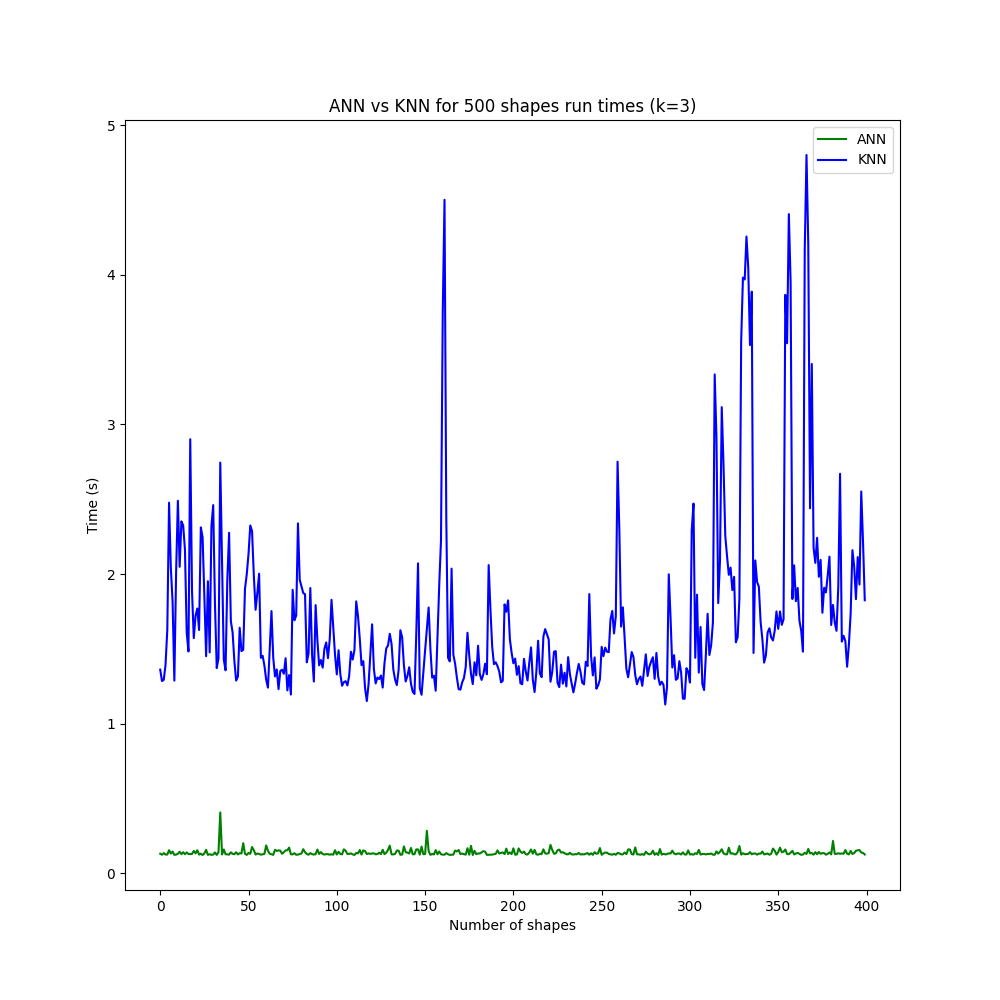
\includegraphics[width = 0.5\textwidth]{assets/evaluation_results/ANN_vs_KNN_run_time.png}
    \caption{ANN vs KNN in terms of run times (k=3)}
    \label{fig:ann-vs-knn-run-times}
\end{figure}


\begin{figure}[H]
    \centering

    \begin{subfigure}[b]{0.3\textwidth}
        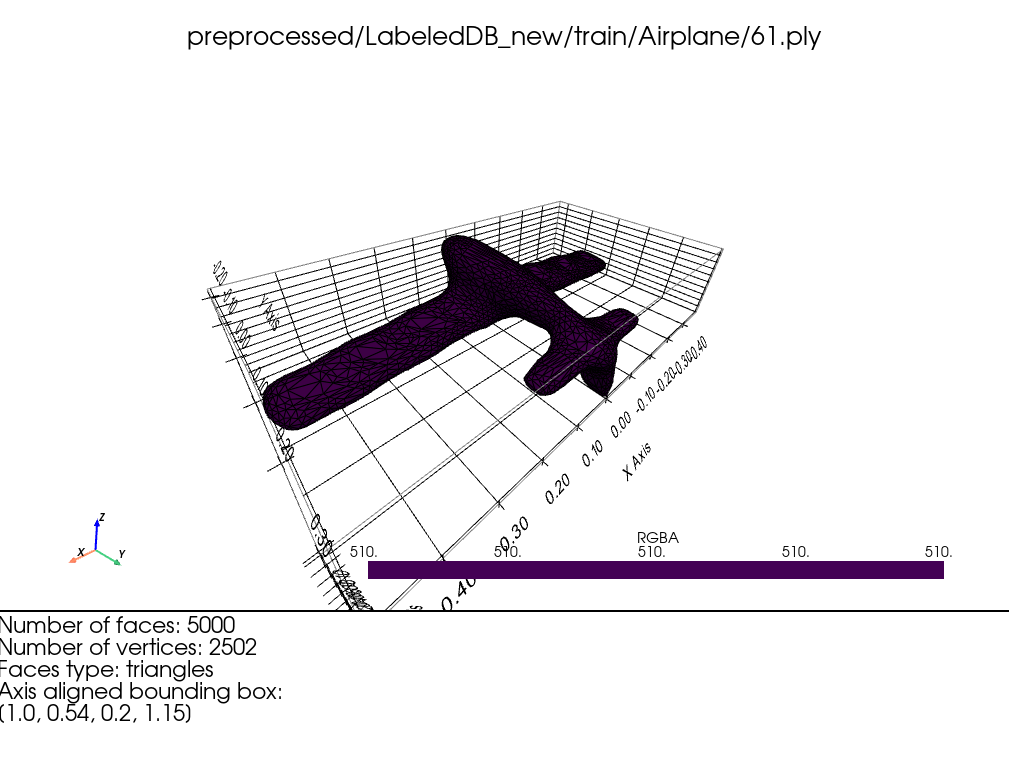
\includegraphics[width=\textwidth]{assets/queries/airplane/input.png}
        \caption{Query input \newline}
        \label{fig:query-input-knn-1}
    \end{subfigure}
    \hfill
    \begin{subfigure}[b]{0.65\textwidth}
        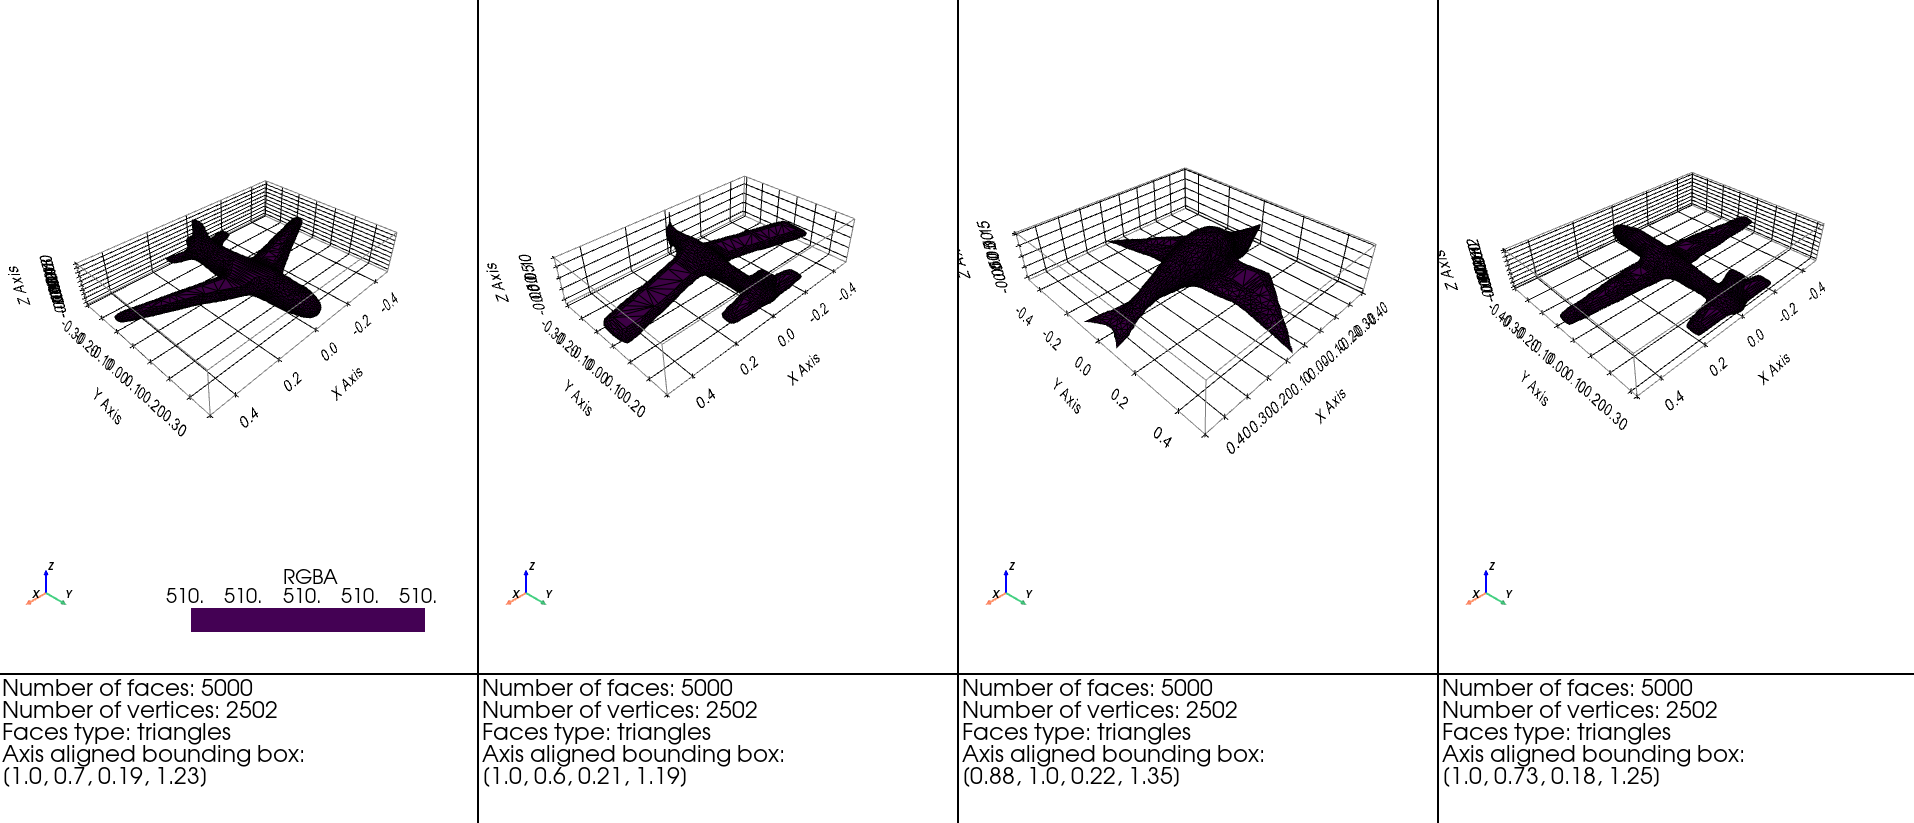
\includegraphics[width=\textwidth]{assets/queries/airplane/output.png}
        \caption{Query output; Respective distances: $7.651\cdot10^{-5}, 8.359\cdot10^{-5}, 9.412\cdot10^{-5}, 10.658\cdot10^{-5}$ }
        \label{fig:query-output-knn-1}
    \end{subfigure}
    \hfill

    \begin{subfigure}[b]{0.3\textwidth}
        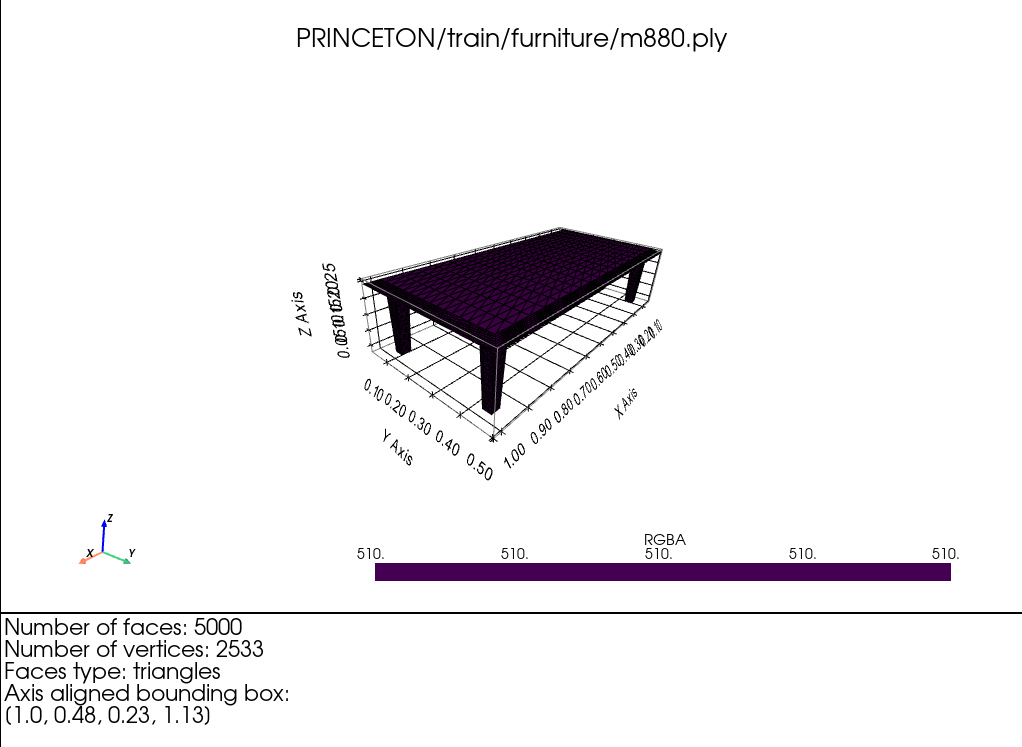
\includegraphics[width=\textwidth]{assets/queries/furniture/input.png}
        \caption{Query input}
        \label{fig:query-input-knn-2}
    \end{subfigure}
    \hfill
    \begin{subfigure}[b]{0.65\textwidth}
        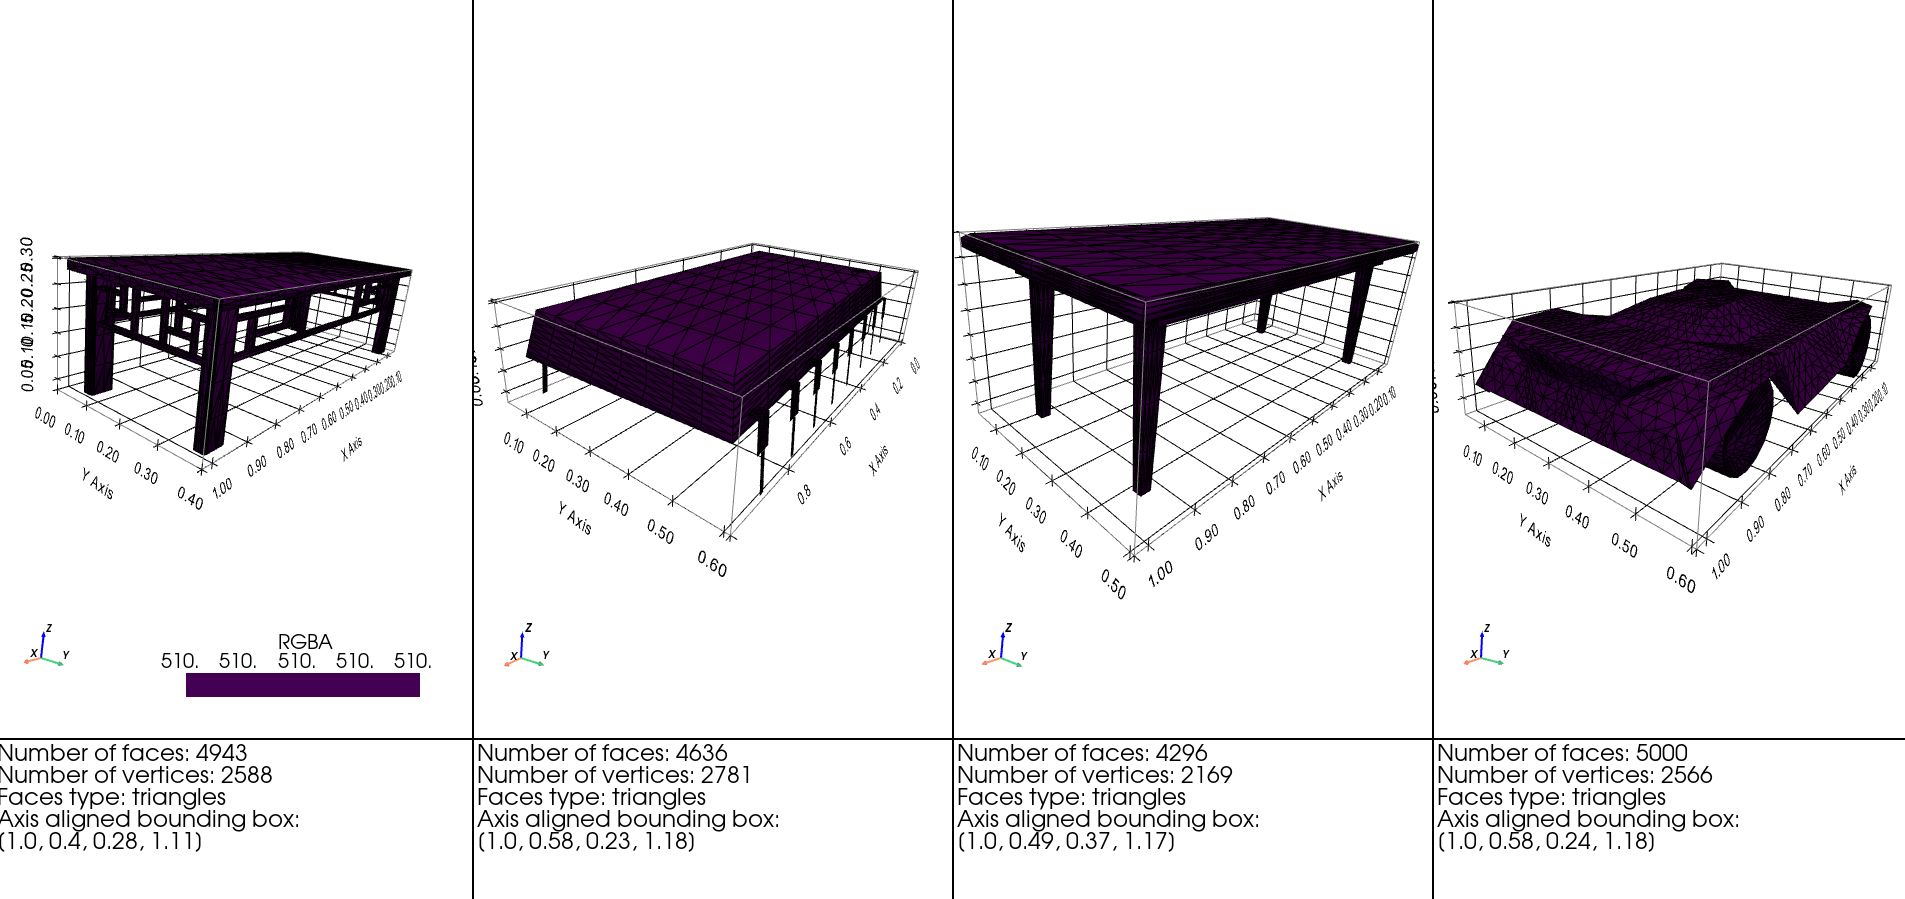
\includegraphics[width=\textwidth]{assets/queries/furniture/output.png}
        \caption{Query output; Respective distances: $ 16.322\cdot10^{-5}, 16.381\cdot10^{-5}, 17.903\cdot10^{-5}, 18.798\cdot10^{-5}$}
        \label{fig:query-output-knn-2}
    \end{subfigure}
    \hfill
    
    \begin{subfigure}[b]{0.3\textwidth}
        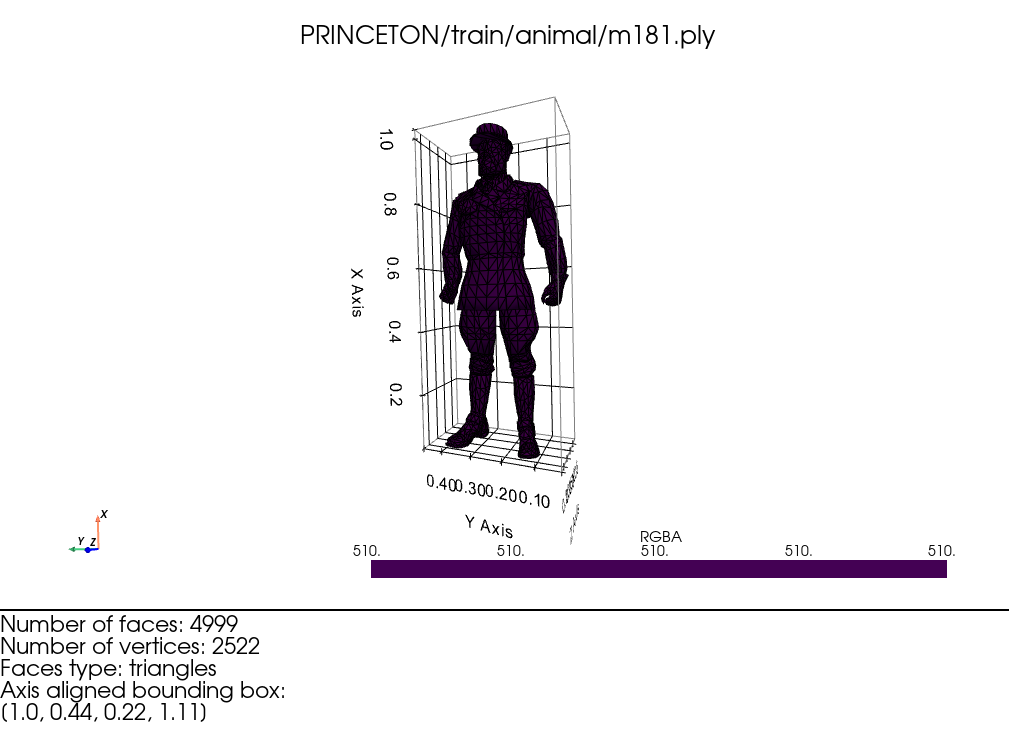
\includegraphics[width=\textwidth]{assets/queries/human/input.png}
        \caption{Query input}
        \label{fig:query-input-knn-3}
    \end{subfigure}
    \hfill
    \begin{subfigure}[b]{0.65\textwidth}
        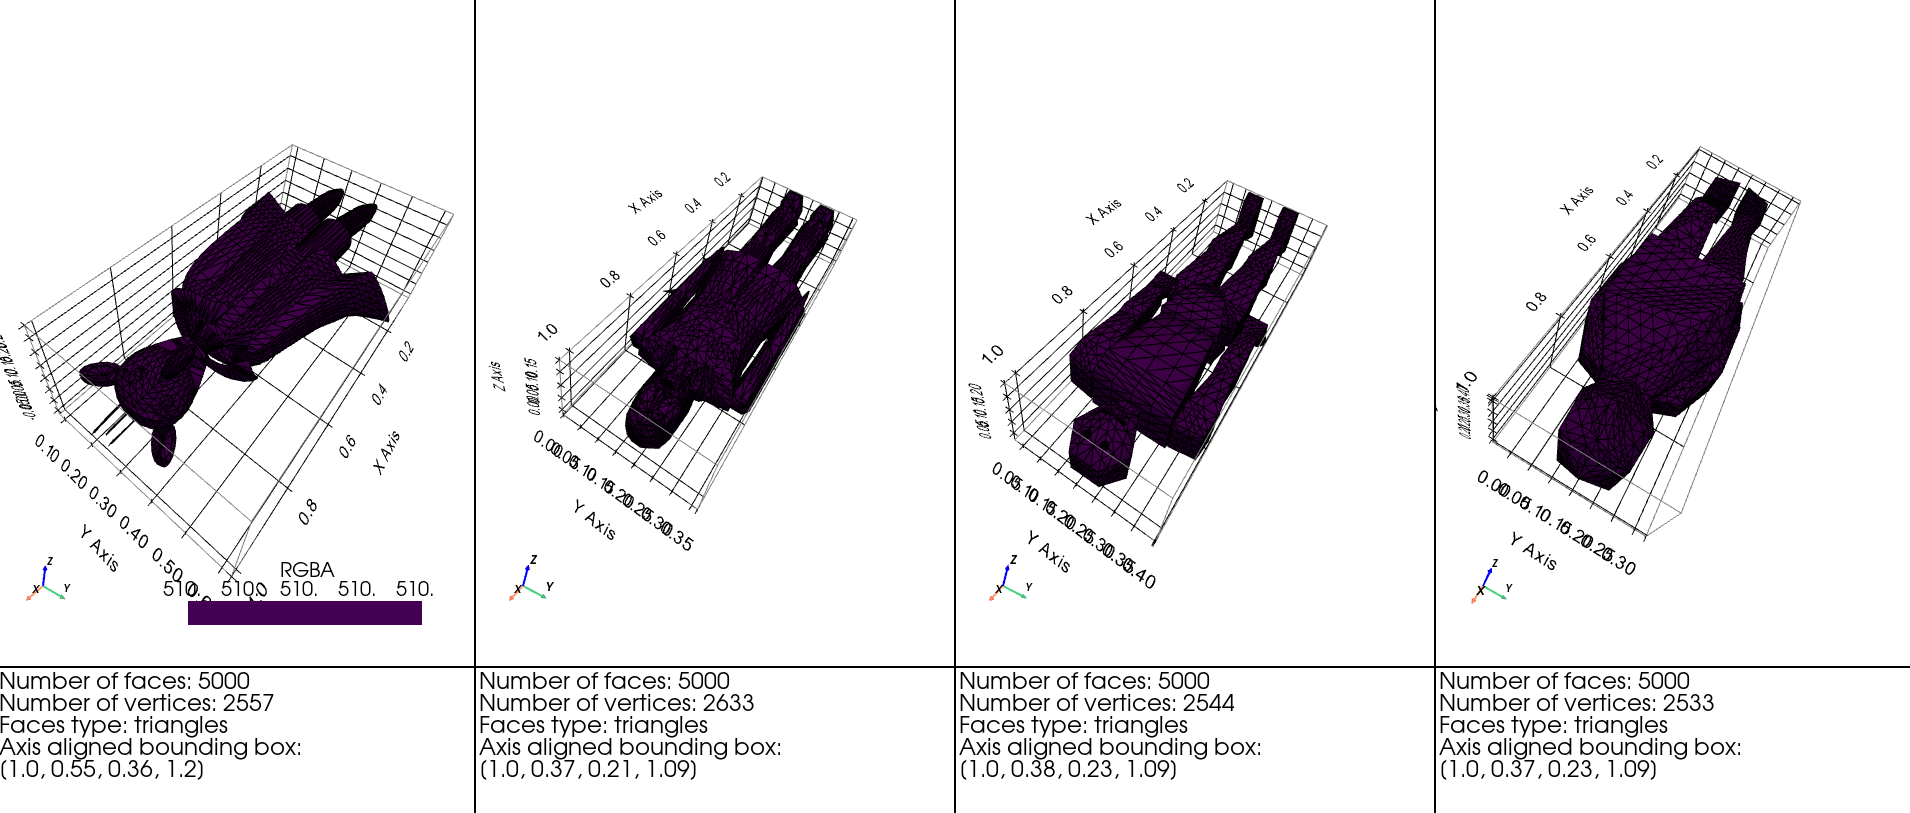
\includegraphics[width=\textwidth]{assets/queries/human/output.png}
        \caption{Query output; Respective distances: $10.354\cdot10^{-5}, 10.799\cdot10^{-5}, 12.264\cdot10^{-5}, 13.187\cdot10^{-5}$}
        \label{fig:query-output-knn-3}
    \end{subfigure}
    \hfill
    
    \caption{Example of the query response using KNN}
    \label{fig:query-response-example}
\end{figure}


\begin{figure}[H]
    \centering
    \begin{subfigure}[b]{0.3\textwidth}
        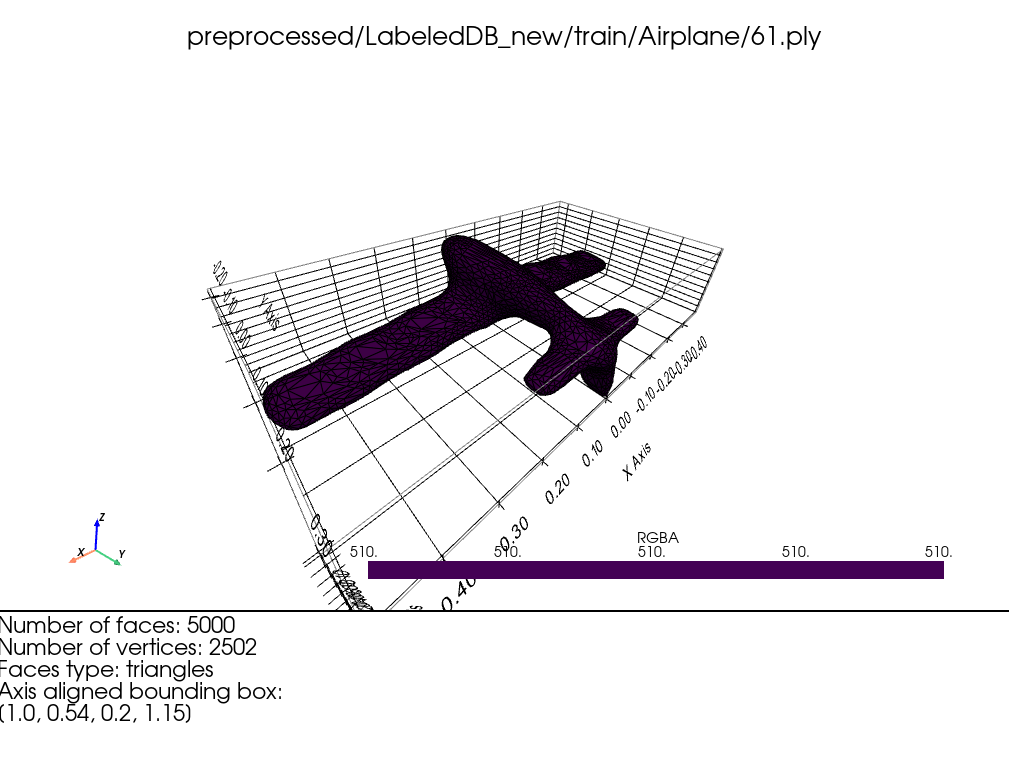
\includegraphics[width=\textwidth]{assets/queries/airplane/input.png}
        \caption{Query input}
        \label{fig:query-input-ann-1}
    \end{subfigure}
    \hfill
    \begin{subfigure}[b]{0.65\textwidth}
        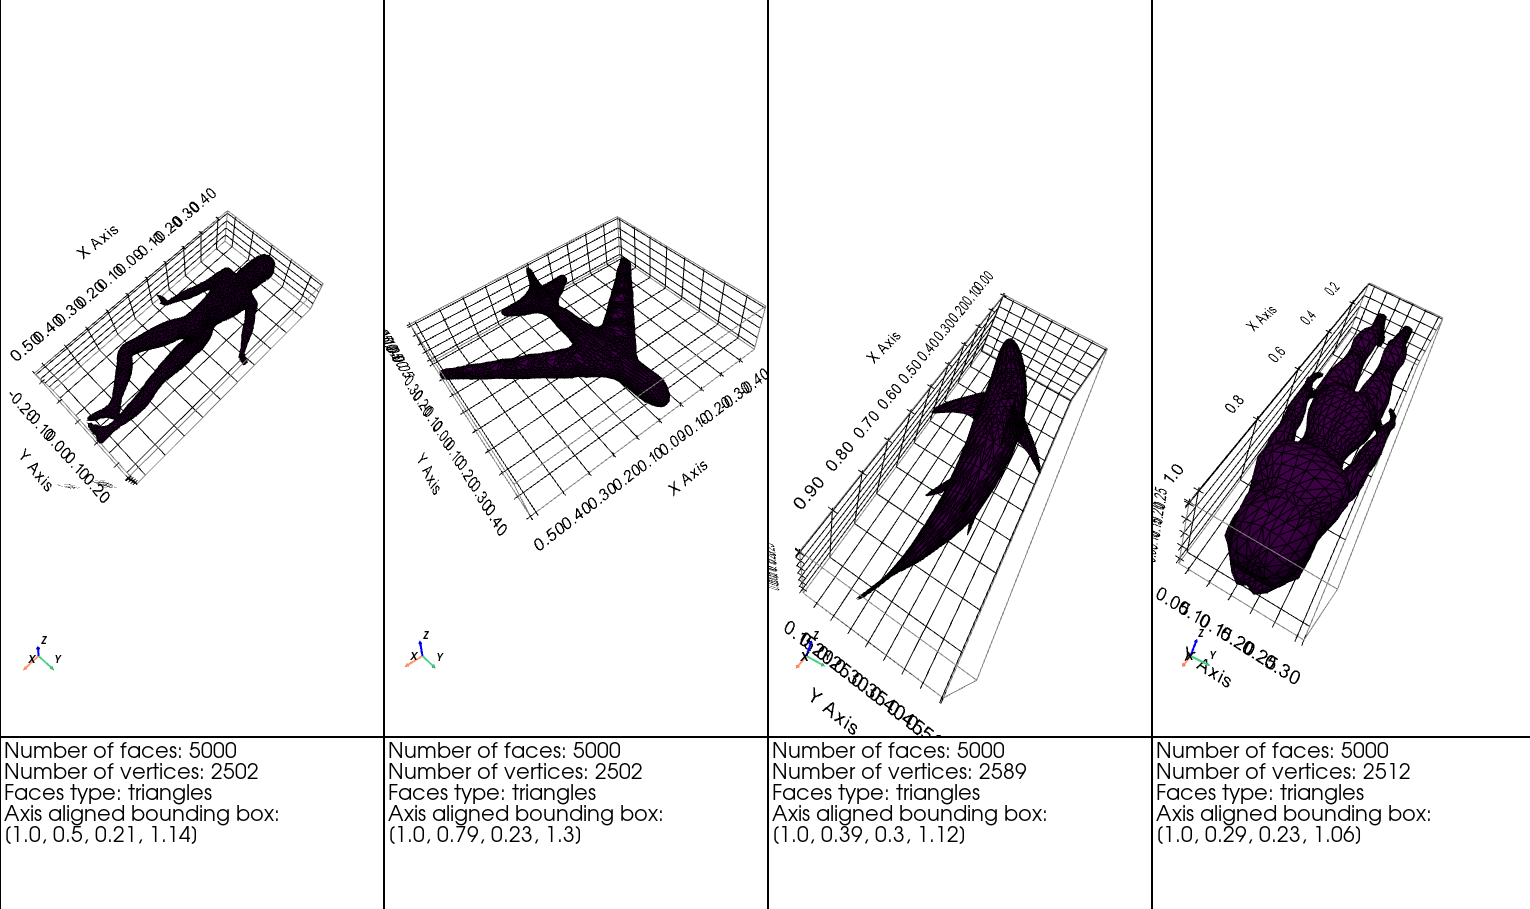
\includegraphics[width=\textwidth]{assets/queries/airplane_ann/output.png}
        \caption{Query output; Respective distances: 0.010, 0.015, 0.018, 0.021}
        \label{fig:query-output-ann-1}
    \end{subfigure}
    \hfill
    
    \begin{subfigure}[b]{0.3\textwidth}
        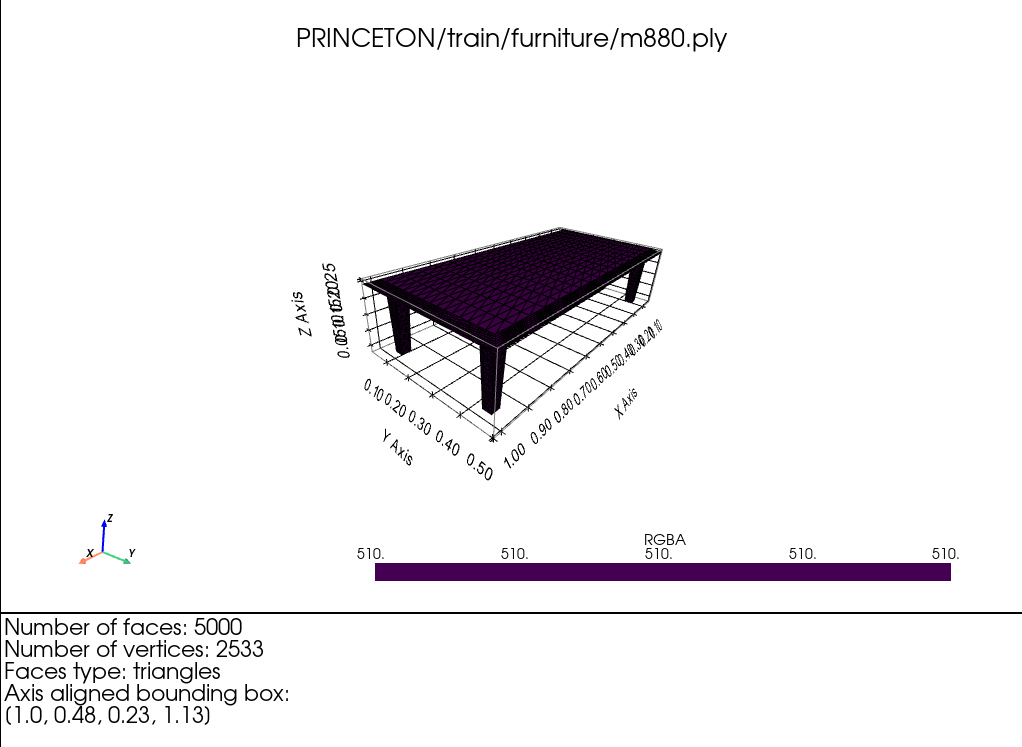
\includegraphics[width=\textwidth]{assets/queries/furniture/input.png}
        \caption{Query input}
        \label{fig:query-input-ann-2}
    \end{subfigure}
    \hfill
    \begin{subfigure}[b]{0.65\textwidth}
        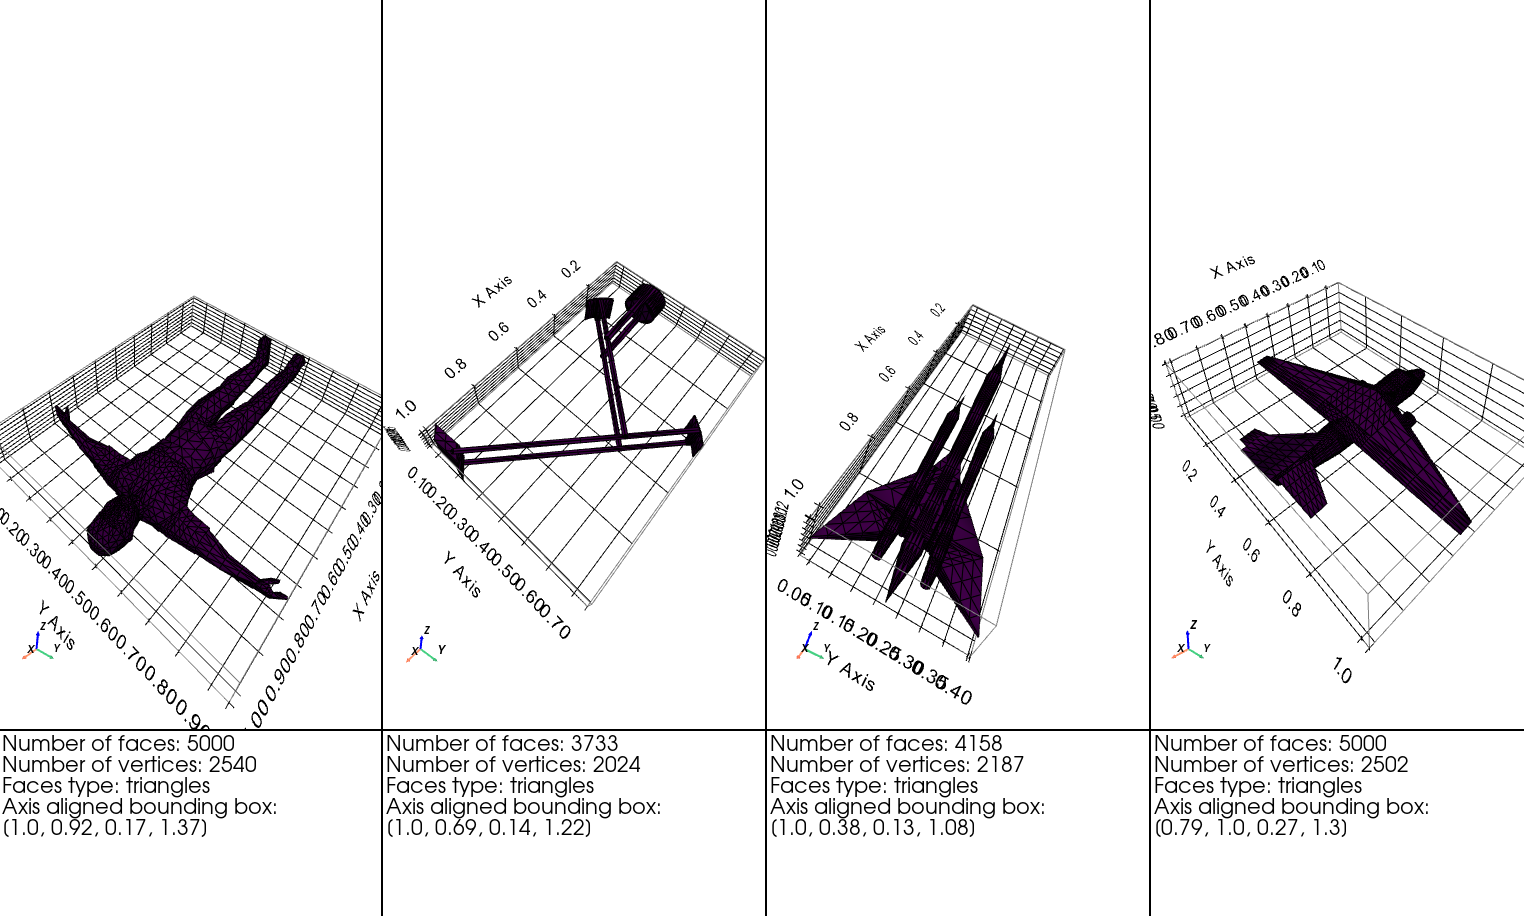
\includegraphics[width=\textwidth]{assets/queries/furniture_ann/output.png}
        \caption{Query output; Respective distances: 0.007, 0.013, 0.015, 0.019}
        \label{fig:query-output-ann-2}
    \end{subfigure}
    \hfill
    
    \begin{subfigure}[b]{0.3\textwidth}
        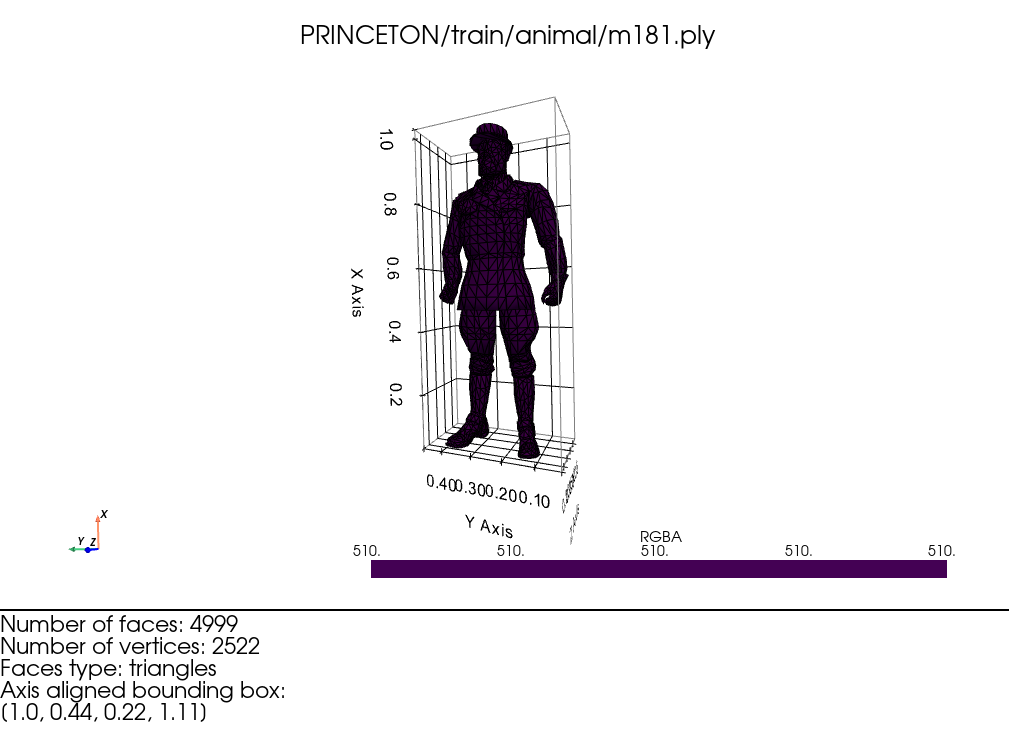
\includegraphics[width=\textwidth]{assets/queries/human/input.png}
        \caption{Query input}
        \label{fig:query-input-ann-3}
    \end{subfigure}
    \hfill
    \begin{subfigure}[b]{0.65\textwidth}
        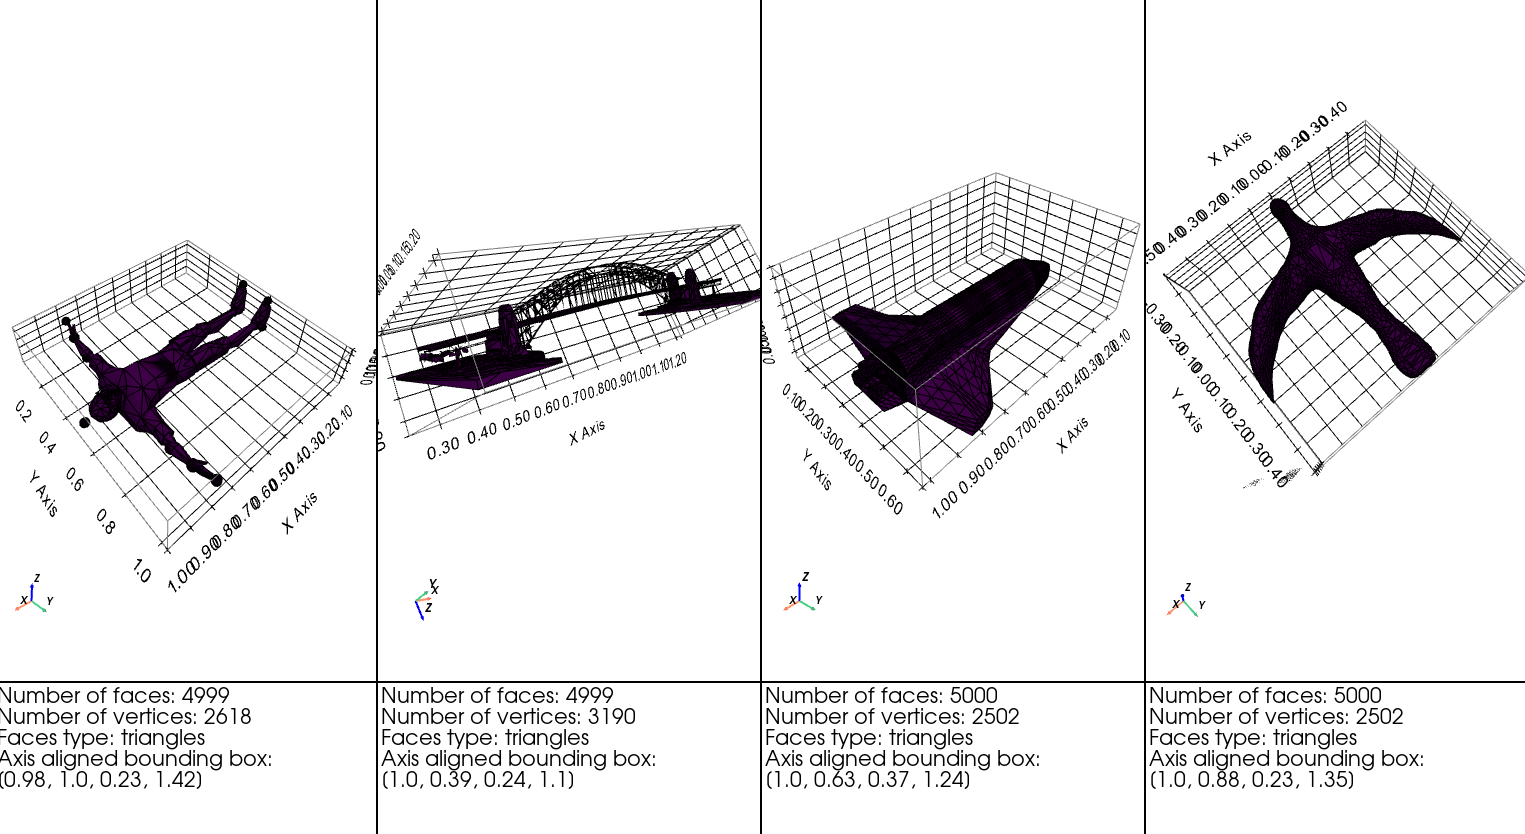
\includegraphics[width=\textwidth]{assets/queries/human_ann/output.png}
        \caption{Query output; Respective distances: 0.0181, 0.0189, 0.0222, 0.0310}
        \label{fig:query-output-ann-3}
    \end{subfigure}
    \hfill
    
    \caption{Example of the query response using ANN}
    \label{fig:query-response-example-ann}
\end{figure}

\begin{figure}[H]
    \centering
    \begin{subfigure}[b]{0.3\textwidth}
        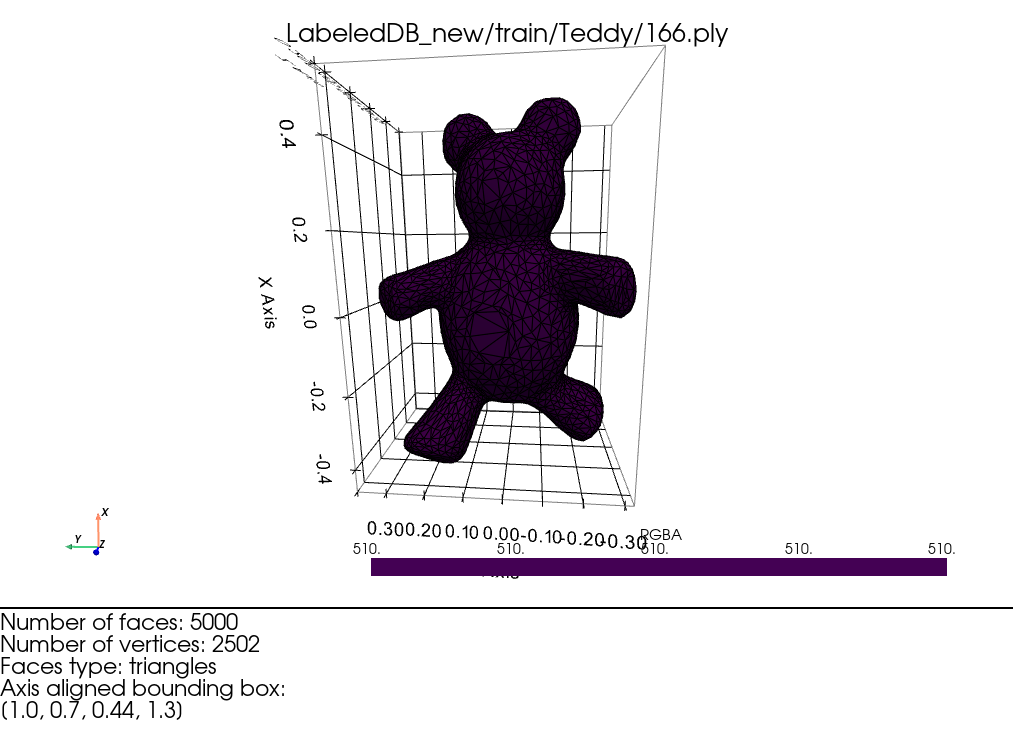
\includegraphics[width=\textwidth]{assets/queries/ann_good/input.png}
        \caption{Query input \newline}
    \end{subfigure}
    \hfill
    \begin{subfigure}[b]{0.65\textwidth}
        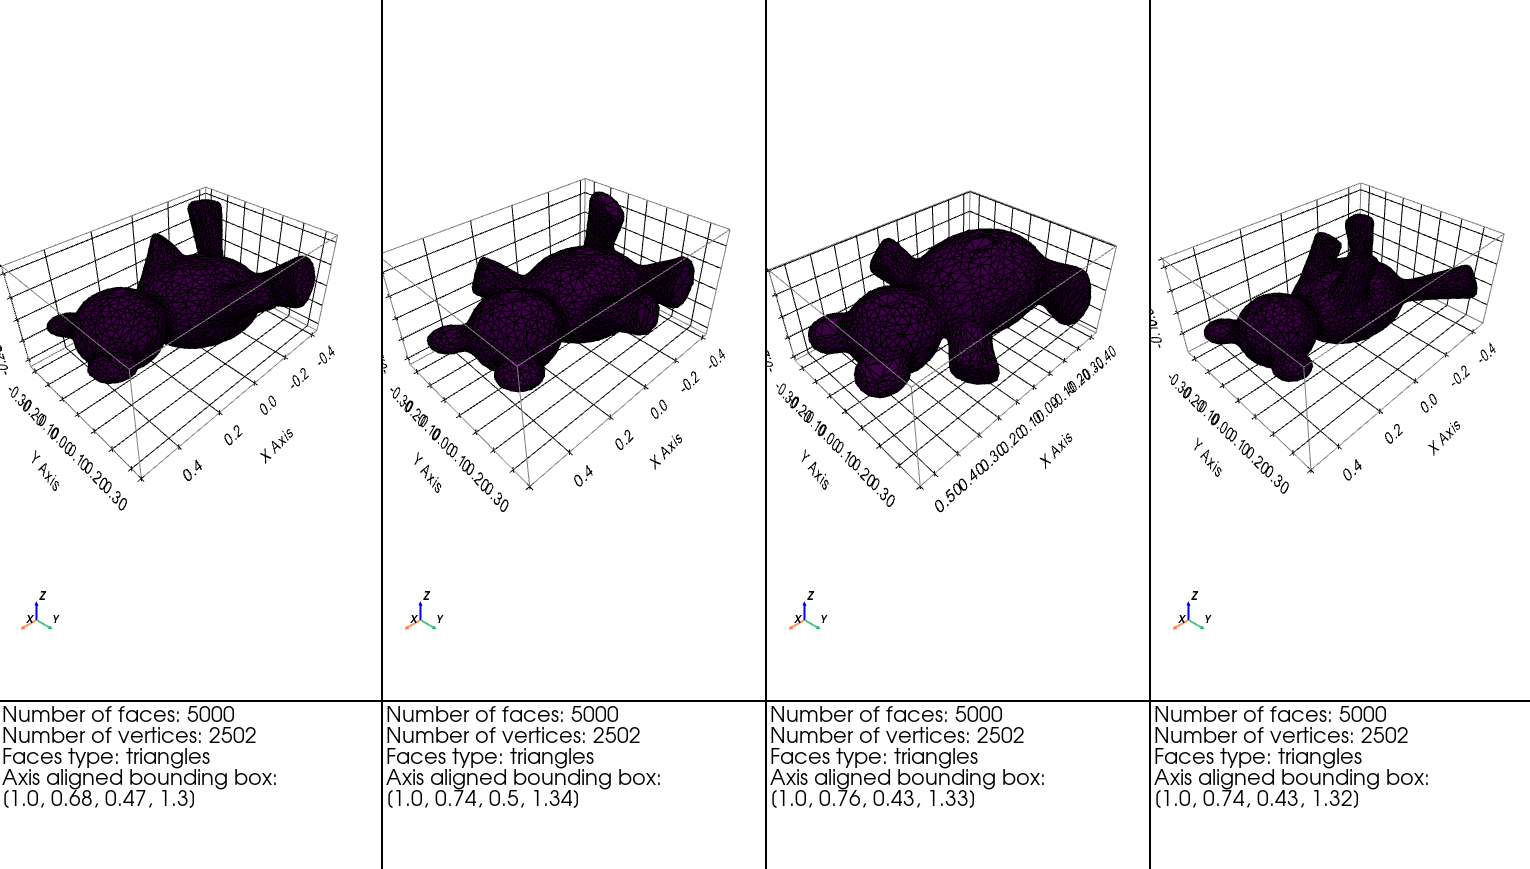
\includegraphics[width=\textwidth]{assets/queries/ann_good/output_ann.png}
        \caption{Query output with ANN; \newline Respective distances: 0.0242, 0.0245, 0.0428, 0.0434}
    \end{subfigure}
    \hfill
    
    \begin{subfigure}[b]{0.3\textwidth}
        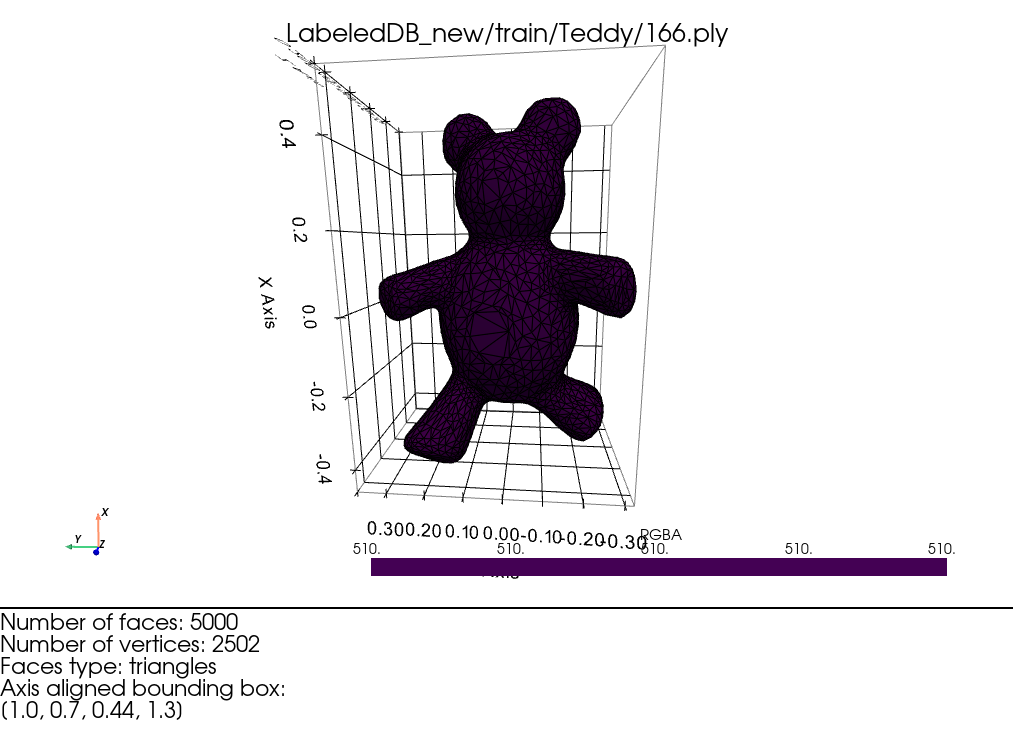
\includegraphics[width=\textwidth]{assets/queries/ann_good/input.png}
        \caption{Query input \newline}
    \end{subfigure}
    \hfill
    \begin{subfigure}[b]{0.65\textwidth}
        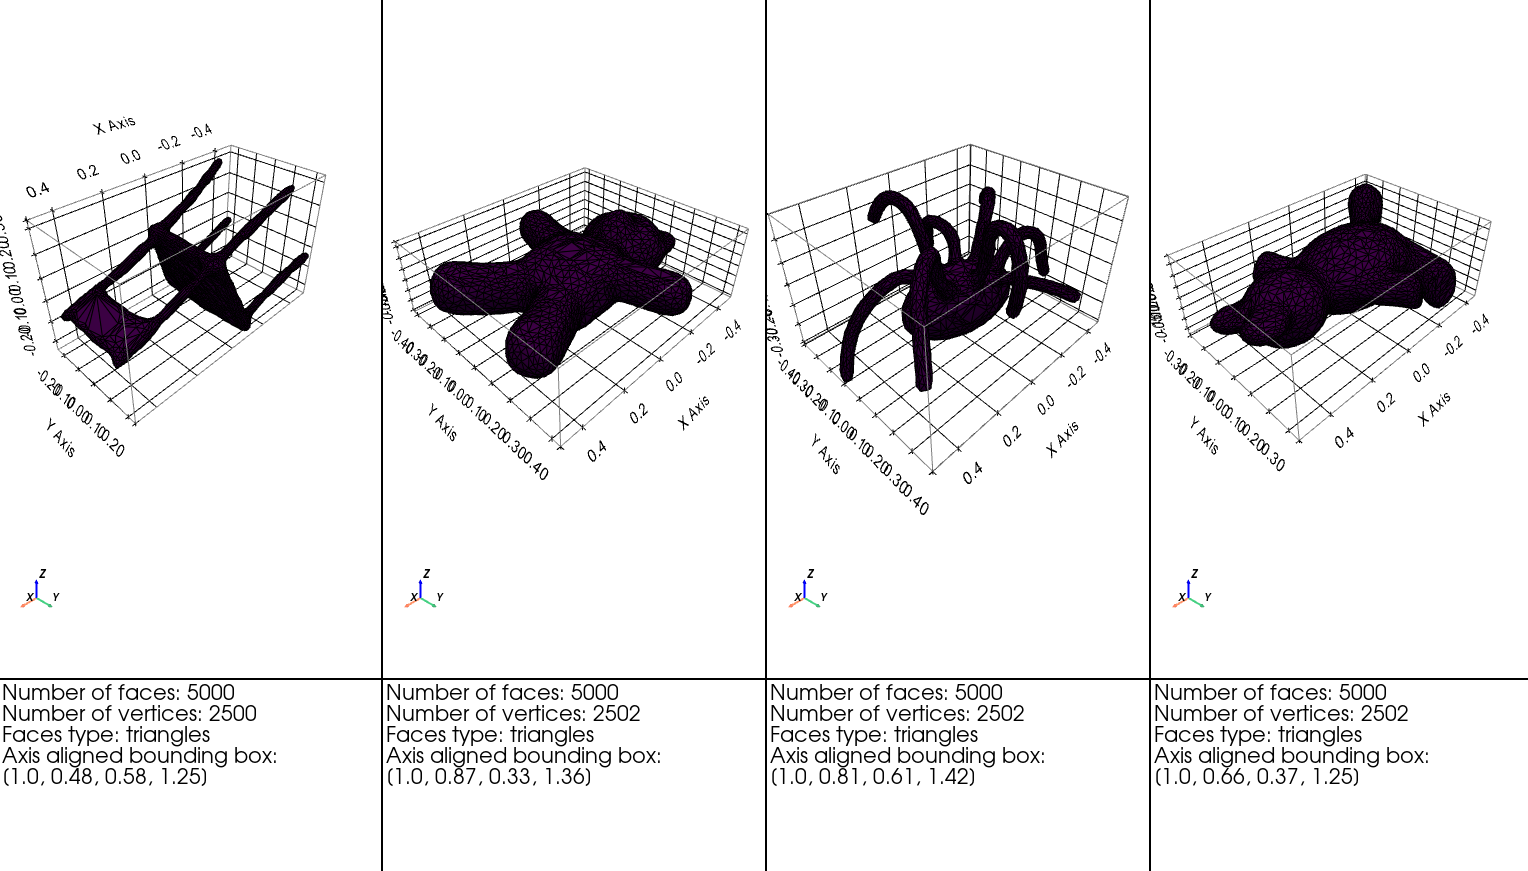
\includegraphics[width=\textwidth]{assets/queries/ann_good/output_knn.png}
        \caption{Query output with KNN;  Respective distances: \newline $10.384\cdot10^{-5}, 10.416\cdot10^{-5}, 10.713\cdot10^{-5}, 10.783\cdot10^{-5}$}
    \end{subfigure}
    \caption{Good example of the query response using ANN vs KNN (with tuned distance functions)}
    \label{fig:query-response-example-ann-good}
\end{figure}

\subsection{Dimensionality reduction}\label{subsec:dimensionality-reduction}
When making a query, the complexity when using a KNN is $O(N \cdot d)$, where $N$ is the number of shapes in the database, and $d$ is the length of their feature vectors.
Dimensionality reduction (DR) techniques aim to reduce the length of $d$, while still preserving as much of the discriminative information as possible.
This would result in smaller - and therefore easier to process, feature vectors, which will reduce the complexity of the querying operation.
While one could design a system which uses the reduced feature vectors for querying, we chose not to explore this approach, considering our ANN approach sufficient.
Instead, we use the technique to visualize the spatial relations of shapes in the database relative to each other.

Consider a feature vector reduction to a size of $2$ across our database.
The reduced vectors can then be plotted in a simple $2D$ plot, where the distance between points represents the difference between different shapes.
The result is shown in Figure (\ref{fig:feature-vectors-2D}).

\paragraph{t-SNE}
To perform the DR, we use an algorithm called t-distributed stochastic neighbour embedding (t-SNE) (see \cite{van2008visualizing} for details).
The algorithm consists of two main stages.
First, a probability distribution over pairs of high-dimensional feature vectors is computed, where similar vectors are assigned a higher probability, while dissimilar ones are assigned a lower one.
In assigning these probabilities, the algorithm uses Gaussian distributions, where the standard deviation is a user-given parameter called $perplexity$.
This parameter indirectly describes the radius of the $n$-dimensional ball centred at a point of the $n$-dimensional space (i.e.\ a feature vector), for which we assign probabilities.
Informally, assigning bigger values for perplexity is useful in sparse data spaces, whilst smaller values are useful in spaces where data is dense.
After the probability distribution for the high-dimensional space is created, a probability distribution is created over the points in the low-dimensional space (i.e.\ 2D) by using a form of $T$-distribution.
To find the new locations in the low-dimension space, the algorithm minimizes the Kullback–Leibler divergence (KL divergence) between the two distributions.

\subsubsection{Results}
Figure \ref{fig:feature-vectors-2D} presents a 2D visualization of our feature vectors with different values for the $perplexity$ parameter.
The technique produces informative results, however a limitation of the resulting is that, due to the fact we have $20$ shape classes, the colours of points can be close and therefore difficult to distinguish.
Also note that the colors of classes are randomly assigned on computation and as a result do not match between the two figures.
Still, there are clear clusters created and there are consistent patterns between Figures \ref{fig:feature-vectors-2D-perplexity-20} and \ref{fig:feature-vectors-2D-perplexity-40}.


The \textit{Mech} and \textit{Plant} classes result in very good clusters in both cases.
Another indication that the technique works well is the fact that clusters from not only within, but also between classes with similar features.
For instance, the \textit{Airplane} and \textit{Bird} classes - which we would expect to have similar features (i.e.\ a large flat area in the wings of both an airplane and a bird).

Still, the results are not perfect.
Notice how in both Figures \ref{fig:feature-vectors-2D-perplexity-20} and \ref{fig:feature-vectors-2D-perplexity-40}, there are some classes (e.g. \textit{vehicle}) tend to not form a cluster.
The feature vectors are rather spread out along the 2D space.
The reason for this is that, in these classes we have shapes that perceptually might be from the same class for a user, but do not share common features.
For instance, the \textit{vehicle} class contains cars, starships, ships, airplanes, tanks, and more.
Conceptually, all of the above are vehicles, but they have very divergent features.

\begin{figure}[H]
    \centering
    \begin{subfigure}[b]{0.55\textwidth}
         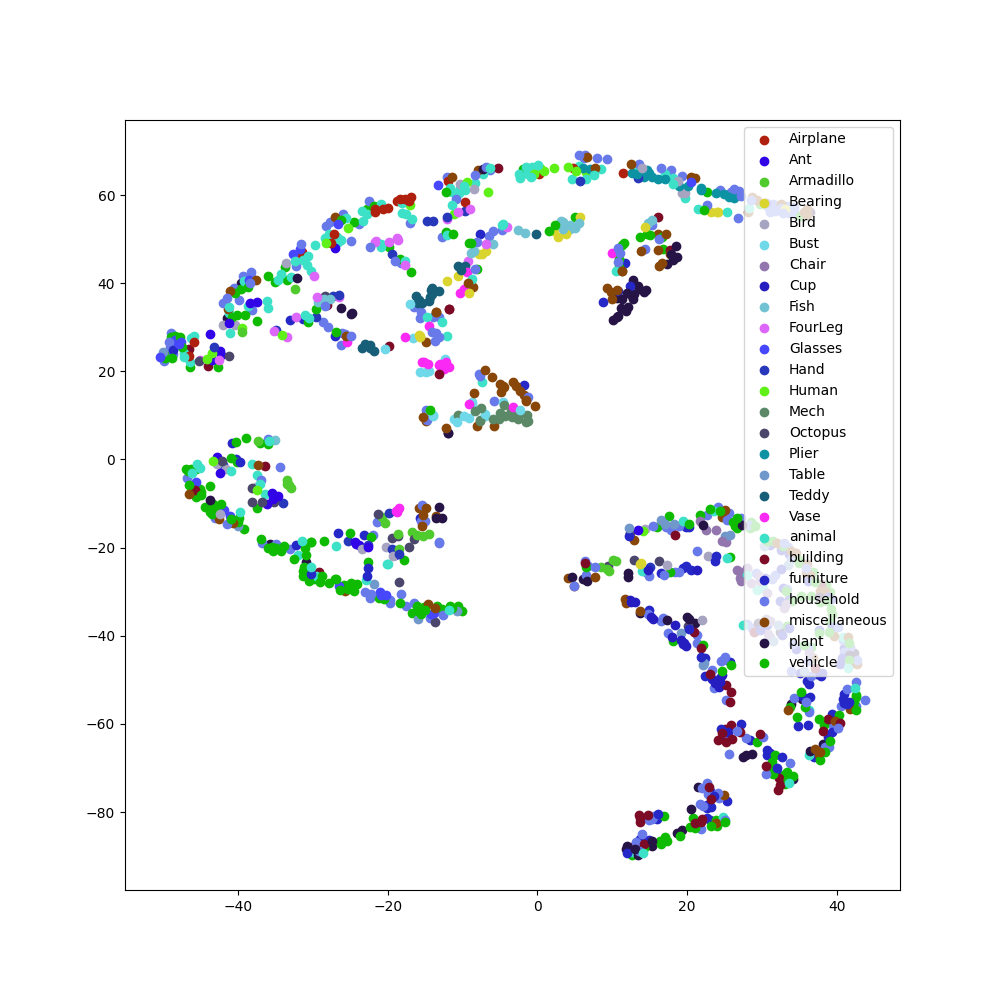
\includegraphics[width=\textwidth]{assets/evaluation_results/tsne_20.png}     
        \caption{$perplexity$=20}
        \label{fig:feature-vectors-2D-perplexity-20}
    \end{subfigure}
    \hfill
    \begin{subfigure}[b]{0.55\textwidth}
         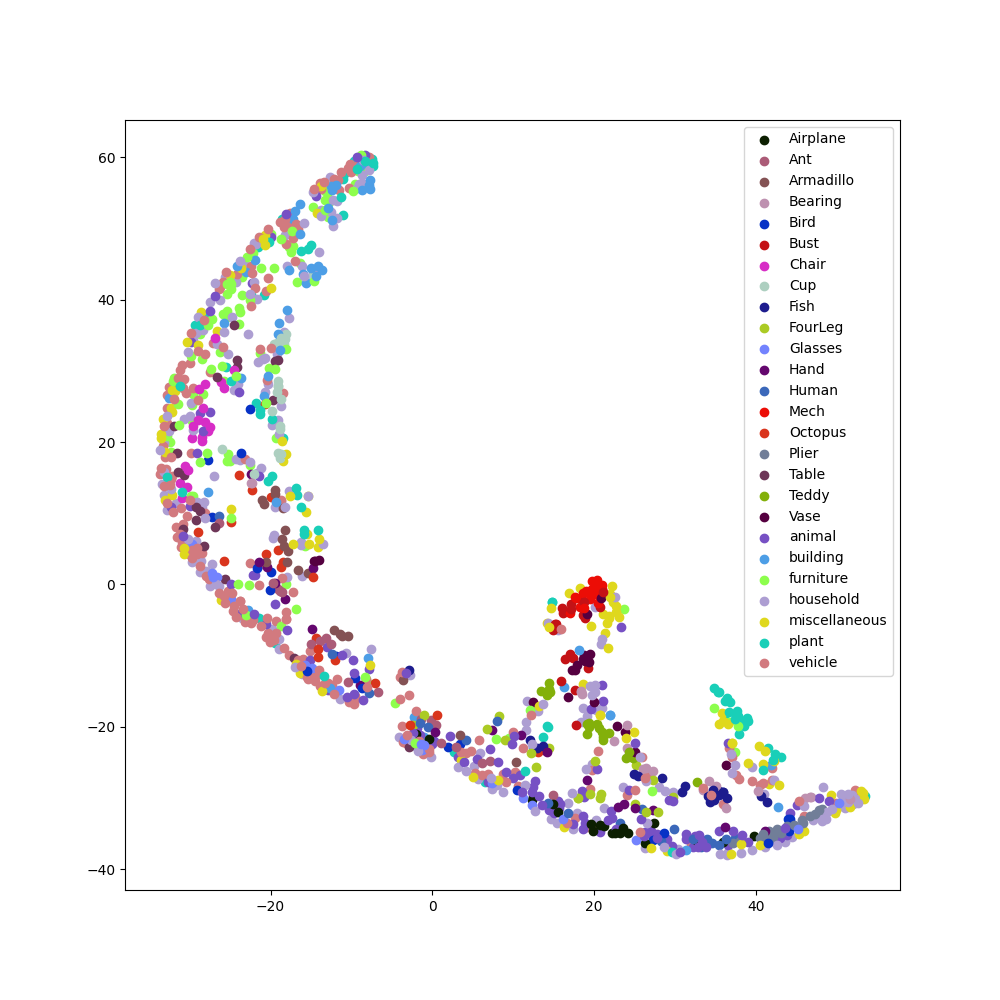
\includegraphics[width=\textwidth]{assets/evaluation_results/tsne_40.png}
         \caption{$perplexity$=40}
         \label{fig:feature-vectors-2D-perplexity-40}
    \end{subfigure}    
    \caption{Feature vectors in 2D}
    \label{fig:feature-vectors-2D}
\end{figure}
